\documentclass[11pt,a4paper]{article}

% ---------- Fonts & encoding ----------
\usepackage[utf8]{inputenc}
\usepackage[T1]{fontenc}
\usepackage{textcomp}
\usepackage{mathptmx}          % Times-like text and math font, Springer-typical
\usepackage{helvet}            % Helvetica for section headings (Springer style)
\usepackage{courier}

% ---------- Page geometry (Springer single-column journal style) ----------
\usepackage[a4paper,left=2.5cm,right=2.5cm,top=2.7cm,bottom=2.8cm,headsep=12pt]{geometry}
\usepackage{setspace}
\onehalfspacing

% ---------- Section heading style ----------
\usepackage{titlesec}
\setcounter{secnumdepth}{-2} % disable auto-numbering; numbers are already in heading text
\titleformat{\section}{\normalfont\sffamily\bfseries\large}{}{0em}{}
\titleformat{\subsection}{\normalfont\sffamily\bfseries\normalsize}{}{0em}{}
\titleformat{\subsubsection}{\normalfont\sffamily\bfseries\itshape\normalsize}{}{0em}{}
\titlespacing*{\section}{0pt}{18pt}{8pt}
\titlespacing*{\subsection}{0pt}{14pt}{6pt}
\titlespacing*{\subsubsection}{0pt}{10pt}{4pt}

% ---------- Tables, math, graphics ----------
\usepackage{amsmath,amssymb}
\usepackage{calc}
\usepackage{longtable}
\usepackage{booktabs}
\usepackage{array}
\usepackage{tikz}
\usetikzlibrary{shapes.geometric,arrows.meta,positioning,fit,backgrounds,plotmarks}
\usepackage{pgfplots}
\pgfplotsset{compat=1.18}
\usepackage{caption}
\captionsetup{font=small,labelfont={sf,bf}}
\usepackage{enumitem}
\setlist[enumerate]{leftmargin=*}
\setlist[itemize]{leftmargin=*}
\providecommand{\tightlist}{\setlength{\itemsep}{0pt}\setlength{\parskip}{0pt}}

% ---------- Misc formatting ----------
\usepackage{xcolor}
\definecolor{springerblue}{RGB}{0,60,113}
\usepackage[colorlinks=true,linkcolor=springerblue,citecolor=springerblue,urlcolor=springerblue]{hyperref}
\usepackage{fancyhdr}
\usepackage{lastpage}

% verbatim / code blocks
\usepackage{fancyvrb}
\fvset{fontsize=\small,frame=single,rulecolor=\color{gray!50},framesep=3mm}
\usepackage{listings}
\lstset{basicstyle=\ttfamily\small,breaklines=true,columns=fullflexible,frame=single,rulecolor=\color{gray!50}}

% Wide tables should still fit in single column
\newcommand{\shrink}[1]{{\small #1}}

% ---------- Unicode glyphs used in the source markdown (math/greek/sub-superscripts) ----------
\usepackage{newunicodechar}
\newunicodechar{°}{\ensuremath{^\circ}}
\newunicodechar{³}{\ensuremath{^3}}
\newunicodechar{α}{\ensuremath{\alpha}}
\newunicodechar{β}{\ensuremath{\beta}}
\newunicodechar{γ}{\ensuremath{\gamma}}
\newunicodechar{μ}{\ensuremath{\mu}}
\newunicodechar{σ}{\ensuremath{\sigma}}
\newunicodechar{⁴}{\ensuremath{^4}}
\newunicodechar{⁵}{\ensuremath{^5}}
\newunicodechar{⁶}{\ensuremath{^6}}
\newunicodechar{⁻}{\ensuremath{^-}}
\newunicodechar{₁}{\ensuremath{_1}}
\newunicodechar{₂}{\ensuremath{_2}}
\newunicodechar{→}{\ensuremath{\rightarrow}}
\newunicodechar{∈}{\ensuremath{\in}}
\newunicodechar{≥}{\ensuremath{\geq}}

% ---------- Headers / footers ----------
\pagestyle{fancy}
\fancyhf{}
\renewcommand{\headrulewidth}{0.4pt}
\renewcommand{\footrulewidth}{0pt}
\fancyhead[L]{\small\sffamily Aether-Eye: Integrated Satellite Intelligence Platform}
\fancyhead[R]{\small\sffamily \thepage}
\fancypagestyle{plain}{%
  \fancyhf{}
  \fancyhead[L]{\small\sffamily Aether-Eye: Integrated Satellite Intelligence Platform}
  \fancyhead[R]{\small\sffamily \thepage}
  \renewcommand{\headrulewidth}{0.4pt}
}

% ---------- Paragraph spacing ----------
\setlength{\parindent}{0pt}
\setlength{\parskip}{6pt}

\begin{document}

% =====================================================================
%  TITLE PAGE  (Springer Nature journal style)
% =====================================================================
\begin{titlepage}
\begin{center}
\vspace*{1.2cm}
 
{\sffamily\bfseries\LARGE Aether-Eye: An Integrated Satellite Intelligence Platform for Automated Critical Infrastructure Monitoring with Multi-Modal OSINT Correlation\par}
 
\vspace{1.4cm}
 
{\normalsize Tanmmay Kanhaiya$^{1}$ \quad Prof. Surendra Reddy Vinta$^{1}$\par}
\vspace{0.4cm}
{\itshape\small $^{1}$School of Computer Science and Engineering, VIT-AP University, Amaravati, Andhra Pradesh, India\par}
 
\vspace{0.5cm}
{\small Corresponding author: \href{mailto:tanmmay.k@vitap.ac.in}{tanmmay.k@vitap.ac.in}\par}

\vspace{1.6cm}

\begin{minipage}{0.85\textwidth}
\centering
{\sffamily\bfseries\normalsize Abstract\par}
\vspace{0.4cm}
\begin{spacing}{1.0}
\small
Satellite-based surveillance of critical infrastructure remains prohibitively expensive and operationally inaccessible for resource-constrained organizations. Commercial imagery platforms such as Maxar and Planet require annual contracts exceeding \$50,000, while manual analyst review cannot scale across dozens of globally distributed sites. This paper presents Aether-Eye, an integrated satellite intelligence platform that combines automated Sentinel-2 scene ingestion via the SpatioTemporal Asset Catalog (STAC) API, deep learning change detection, fine-grained military aircraft classification, ADS-B flight activity tracking, and open-source intelligence (OSINT) correlation into a single unified pipeline. The system employs a SiameseUNet architecture for multi-temporal change detection, achieving a test Intersection-over-Union (IoU) of 0.8243 on paired building-change satellite tiles. A ConvNeXt Small classifier fine-tuned on a 98-class military aircraft dataset covering 34,718 training chips achieves 68.57\% top-1 validation accuracy using a novel two-phase transfer learning methodology with layer-wise learning rate scheduling. INT8 dynamic quantization compresses the combined model footprint from 314~MB to 81~MB (3.7--3.96$\times$ compression) with less than 1\% accuracy degradation, enabling deployment within 512~MB free-tier cloud RAM constraints. A three-pass scored geo-tagging algorithm correlates articles from 21 curated RSS sources to 18 globally monitored sites, achieving a 24.7\% article-to-site match rate. The complete system is deployable at zero recurring cost using Vercel, Render, and Supabase free tiers, demonstrating that the gap between research-grade machine learning and operationally deployable intelligence tools can be addressed through systematic integration of freely available satellite data, open-source models, and aggressive model compression.
\end{spacing}

\vspace{0.5cm}
{\small\textbf{Keywords:} satellite imagery, change detection, Siamese networks, aircraft classification, ConvNeXt, OSINT, geospatial intelligence, critical infrastructure, Sentinel-2, ONNX, edge deployment\par}
\end{minipage}

\vfill
{\footnotesize Working draft --- prepared for advisor review and journal submission (target venue: IEEE Access / Remote Sensing MDPI)\par}
\end{center}
\end{titlepage}

\setcounter{page}{1}
\hypertarget{introduction}{%
\section{1. Introduction}\label{introduction}}

Satellite-based monitoring of critical infrastructure---military airbases, naval installations, strategic ports, and civil airports---is a cornerstone of modern geospatial intelligence (GEOINT). Nation-states and defense organizations rely on persistent overhead surveillance to detect construction activity, track aircraft deployments, monitor naval vessel movements, and identify anomalous patterns that may indicate shifting military postures. However, the operational landscape is dominated by commercial providers whose pricing models place continuous monitoring beyond the reach of independent researchers, allied partner nations with limited defense budgets, and academic institutions studying conflict dynamics.

Commercial satellite imagery platforms illustrate this accessibility gap. Maxar Technologies offers sub-meter resolution tasking at costs exceeding \$50,000 per year for programmatic access. Planet Labs provides daily global coverage at 3--5 m resolution through its SkySat and PlanetScope constellations, but similarly requires substantial subscription commitments. Even when imagery is acquired, the analysis bottleneck persists: trained imagery analysts manually review scenes, a process that does not scale when monitoring dozens of geographically distributed sites simultaneously.

The European Space Agency's Copernicus Sentinel-2 mission fundamentally changes this cost equation. Sentinel-2 provides free, open-access multispectral imagery at 10 m/pixel spatial resolution with a 5-day revisit cycle at the equator. The SpatioTemporal Asset Catalog (STAC) specification [10] enables programmatic discovery and retrieval of scenes through standardized API queries, eliminating the need for manual data procurement. Simultaneously, deep learning has matured to the point where convolutional neural networks achieve deployment-ready accuracy for both pixel-level change detection {[}1, 2, 3{]} and fine-grained visual classification {[}4, 5{]}, with model compression techniques enabling inference on resource-constrained hardware.

Despite these advances, a significant gap exists in the literature: no published system combines all of the following capabilities within a single unified, self-hosted platform: (a) automated satellite scene ingestion from open data sources, (b) Siamese network change detection for temporal comparison, (c) fine-grained military aircraft classification spanning nearly 100 airframe variants, (d) OSINT news correlation geo-tagged to specific monitored sites, and (e) ADS-B flight activity baselines for aerial traffic pattern analysis. Existing systems address individual components in isolation---change detection benchmarks evaluate model accuracy without operational pipelines, OSINT aggregators like GDELT [8] lack satellite integration, and aircraft classifiers train on civilian photography without military-specific taxonomy.

This paper presents Aether-Eye, an end-to-end satellite intelligence platform that addresses this integration gap. Our contributions are:

\begin{enumerate}
\def\labelenumi{\arabic{enumi}.}
\tightlist
\item
  An \textbf{end-to-end automated pipeline} from STAC discovery through change detection, event generation, temporal baseline anomaly scoring, and multi-channel alerting.
\item
  A \textbf{SiameseUNet change detection model} trained on 1,134 paired satellite tiles achieving a test IoU of 0.8243, competitive with published methods on comparable datasets.
\item
  A \textbf{ConvNeXt Small military aircraft classifier} covering 98 distinct airframe variants across 34,718 training chips, achieving 68.57\% top-1 accuracy via a two-phase fine-tuning protocol with 10$\times$ layer-wise learning-rate scheduling that prevents catastrophic forgetting of pretrained backbone features---uniform learning rate in Phase 2 collapses accuracy to 7.5\% at epoch 1, while layer-wise decay recovers and ultimately exceeds the head-only baseline, reaching 68.57\%.
\item
  A \textbf{three-pass scored OSINT geo-tagging algorithm} correlating 21 curated RSS sources to 18 globally monitored sites using tag matching, alias resolution, and country-military context boosting.
\item
  \textbf{INT8 dynamic quantization} achieving 3.7--3.96× model compression, reducing the total inference footprint to 81 MB for free-tier cloud deployment within 512 MB RAM constraints.
\item
  A \textbf{complete open-source system} deployable via a single \texttt{docker\ compose} command at zero recurring cost.
\end{enumerate}

\hypertarget{related-work}{%
\section{2. Related Work}\label{related-work}}

\hypertarget{satellite-change-detection}{%
\subsection{2.1 Satellite Change Detection}\label{satellite-change-detection}}

Siamese network architectures have established themselves as the dominant paradigm for remote sensing change detection. Daudt et al.~[1] introduced Fully Convolutional Siamese Networks (FC-Siam-Conc and FC-Siam-Diff), demonstrating that shared-weight encoders processing bi-temporal image pairs can effectively learn change representations without explicit feature engineering. The LEVIR-CD dataset [2] subsequently became the standard benchmark, comprising 637 pairs of 1024×1024 pixel Google Earth images annotated for building change. State-of-the-art methods on LEVIR-CD report IoU scores between 0.83 and 0.87, with transformer-based architectures such as ChangeFormer [3] achieving 0.823 IoU by incorporating self-attention mechanisms for long-range spatial dependencies.

Our SiameseUNet architecture follows the FC-Siam-Diff paradigm with a U-Net decoder, achieving 0.8243 test IoU on the Building-change dataset---a comparable-scale benchmark to LEVIR-CD. While not directly comparable due to dataset differences, this result indicates competitive performance with published methods using a substantially simpler convolutional architecture amenable to INT8 quantization and edge deployment.

\hypertarget{fine-grained-aircraft-classification}{%
\subsection{2.2 Fine-Grained Aircraft Classification}\label{fine-grained-aircraft-classification}}

Fine-Grained Visual Classification (FGVC) of aircraft was formalized by Maji et al.~[5], who introduced the FGVC-Aircraft benchmark containing 10,000 images across 100 aircraft variant classes. ResNet-50 baselines achieve approximately 88\% top-1 accuracy on this dataset under standard training protocols. The ConvNeXt family [4] modernized convolutional architectures by incorporating design elements from Vision Transformers---patchify stems, depthwise separable convolutions, inverted bottleneck blocks, and GELU activations---achieving competitive accuracy with ViT-Base while maintaining favorable inference latency (40--50 ms vs.~90--120 ms on GPU).

A critical challenge unaddressed in the literature is the domain shift between oblique photography (the standard capture geometry for FGVC-Aircraft) and nadir satellite imagery. No published work specifically addresses 98-class military aircraft classification on a dataset combining nadir and oblique views, which Aether-Eye's v2 classifier targets.

\hypertarget{osint-and-geospatial-intelligence-systems}{%
\subsection{2.3 OSINT and Geospatial Intelligence Systems}\label{osint-and-geospatial-intelligence-systems}}

The Global Database of Events, Language, and Tone (GDELT) [8] monitors global news media in over 100 languages, extracting events, actors, and sentiment at planetary scale. GDELT's event taxonomy classifies over 300 event types using the CAMEO coding scheme, enabling longitudinal analysis of geopolitical dynamics. However, GDELT operates as a general-purpose event database without integration into satellite anomaly detection workflows---it cannot, for example, correlate a ``military deployment'' event with construction activity detected in overhead imagery of the same facility.

Commercial systems such as Pharos-AI and Recorded Future combine OSINT with threat intelligence feeds, but their pricing models (\$100k+/year) target enterprise and government customers. Academic prototypes such as WorldMonitor and the IARPA-funded CAUSE program have explored event prediction from open-source data, but these systems focus on forecasting rather than real-time operational monitoring. The IARPA Open Source Indicators (OSI) program demonstrated that combining diverse open-source signals improves event detection, but did not incorporate satellite imagery as an input modality.

Aether-Eye bridges this integration gap by geo-tagging OSINT articles directly to the same 18 sites monitored by its satellite and ADS-B subsystems. This enables a unique analytical capability: an operator can observe, on a single dashboard, that Bandar Abbas Port shows increased vessel activity in Sentinel-2 imagery, elevated ADS-B flight counts, and a cluster of OSINT articles mentioning IRGC Naval exercises---providing multi-modal corroboration that no single-modality system can achieve.

\hypertarget{edge-and-resource-constrained-deployment}{%
\subsection{2.4 Edge and Resource-Constrained Deployment}\label{edge-and-resource-constrained-deployment}}

Deploying deep learning models on resource-constrained platforms has received increasing attention as the gap between research-grade GPU clusters and operational edge environments remains significant. Model compression techniques fall into several categories: pruning (removing low-magnitude weights), knowledge distillation (training smaller student models from larger teacher models), and quantization (reducing numerical precision from FP32 to INT8 or lower).

INT8 quantization is particularly attractive for deployment scenarios because it reduces model size by approximately 4× while leveraging hardware-accelerated integer arithmetic available on modern CPUs. ONNX Runtime provides a unified inference execution framework across CPU and GPU backends with built-in support for both static (calibration-based) and dynamic (weight-only) quantization. Dynamic quantization requires no calibration dataset and can be applied post-training as a single export step.

A practical constraint not typically addressed in the change detection or FGVC literature is deployment on free-tier cloud platforms. Services such as Render, Koyeb, and Railway offer 512 MB RAM instances at zero cost, but this imposes hard limits on model size, runtime memory, and concurrent inference. Aether-Eye leverages dynamic INT8 quantization to compress its model portfolio from 314 MB to 81 MB, enabling deployment within these constraints---demonstrating that research-grade models can be operationalized without dedicated GPU infrastructure or paid cloud services.

\hypertarget{system-architecture}{%
\section{3. System Architecture}\label{system-architecture}}

\hypertarget{overview}{%
\subsection{3.1 Overview}\label{overview}}

Aether-Eye is organized as a four-layer architecture separating data ingestion, model inference, intelligence synthesis, and visualization concerns, as summarized in Figure~\ref{fig:architecture}.

\begin{figure}[t]
\centering
\resizebox{\columnwidth}{!}{\documentclass[tikz,border=5pt]{standalone}

% ---------- Packages ----------
\usepackage[T1]{fontenc}
\usepackage{tikz}
\usetikzlibrary{arrows.meta, shapes.geometric, fit, backgrounds,
                positioning, calc, decorations.pathrounding}

% ---------- Custom Styles ----------

% Data source box (Layer 1 — blue)
\tikzstyle{datasrc} = [rectangle, rounded corners=3pt,
  minimum width=2.8cm, minimum height=0.7cm,
  draw=blue!60!black, fill=blue!10,
  font=\small\ttfamily, align=center, text=black]

% Model box (Layer 2 — green)
\tikzstyle{modelbox} = [rectangle, rounded corners=3pt,
  minimum width=3cm, minimum height=0.8cm,
  draw=green!50!black, fill=green!10,
  font=\small\bfseries, align=center, text=black]

% Intel box (Layer 3 — purple)
\tikzstyle{intelbox} = [rectangle, rounded corners=3pt,
  minimum width=3cm, minimum height=0.7cm,
  draw=purple!60!black, fill=purple!10,
  font=\small, align=center, text=black]

% Viz box (Layer 4 — red)
\tikzstyle{vizbox} = [rectangle, rounded corners=3pt,
  minimum width=3cm, minimum height=0.7cm,
  draw=red!60!black, fill=red!10,
  font=\small, align=center, text=black]

% Layer band label
\tikzstyle{bandlabel} = [rectangle, rounded corners=2pt, fill=gray!20,
  draw=gray!50, font=\footnotesize\bfseries\sffamily,
  minimum width=1.8cm, align=center, inner sep=3pt]

% Arrow styles
\tikzstyle{arr} = [-{Stealth[length=4pt]}, thick, gray!70]
\tikzstyle{darr} = [-{Stealth[length=4pt]}, thick, black!70]
\tikzstyle{dbarr} = [-{Stealth[length=4pt]}, thick, orange!70!black]

\begin{document}
\begin{tikzpicture}[node distance=0.5cm]

% =====================================================================
%  LAYER 1 — DATA INGESTION
% =====================================================================
\node[bandlabel] (L1label) at (-6.2, 5) {LAYER 1\\DATA\\INGESTION};

% --- Satellite pipeline (top row) ---
\node[datasrc] (A1) at (-4.2, 6) {Copernicus STAC\\Sentinel-2 L2A};
\node[datasrc] (A2) at (-0.8, 6) {STAC Watcher\\{\scriptsize (6\,hr schedule)}};
\node[datasrc] (A3) at (2.6,  6) {Scene Processor\\GeoTIFF Tiler};
\node[datasrc] (A4) at (6.0,  6) {512$\times$512 tiles\\{\scriptsize (rasterio)}};

\draw[arr] (A1) -- (A2);
\draw[arr] (A2) -- (A3);
\draw[arr] (A3) -- (A4);

% --- ADS-B pipeline (middle row) ---
\node[datasrc] (B1) at (-4.2, 4.8) {OpenSky Network\\ADS-B API};
\node[datasrc] (B2) at (-0.8, 4.8) {Flight Poller\\{\scriptsize (5\,min)}};
\node[datasrc] (B3) at (2.6,  4.8) {flight\_states\\table};

\draw[arr] (B1) -- (B2);
\draw[arr] (B2) -- (B3);

% --- OSINT pipeline (bottom row) ---
\node[datasrc] (C1) at (-4.2, 3.6) {21 RSS Sources\\{\scriptsize BBC\,\textperiodcentered\,AJ\,\textperiodcentered\,DefNews}};
\node[datasrc] (C2) at (-0.8, 3.6) {OSINT Ingestor\\{\scriptsize (30\,min)}};
\node[datasrc] (C3) at (2.6,  3.6) {intel\_articles\\table};

\draw[arr] (C1) -- (C2);
\draw[arr] (C2) -- (C3);

% --- Layer 1 background band ---
\begin{scope}[on background layer]
  \node[draw=blue!40!black, dashed, rounded corners=6pt,
        fill=blue!4, inner sep=8pt,
        fit=(A1)(A4)(C1)(C3)] (L1band) {};
\end{scope}

% =====================================================================
%  CENTRAL DATABASE
% =====================================================================
\node[cylinder, shape border rotate=90,
      draw=orange!80!black, fill=orange!15,
      minimum width=3.6cm, minimum height=0.9cm,
      font=\small\bfseries, align=center,
      aspect=0.2] (DB) at (1.0, 2.4)
      {PostgreSQL 16 + PostGIS 3.4};

% Arrows from Layer 1 down into DB
\draw[dbarr] (A4.south) -- ++(0,-0.4) -| (DB.20);
\draw[dbarr] (B3.south) -- ++(0,-0.3) -| (DB.160);
\draw[dbarr] (C3.south) -- ++(0,-0.2) -| (DB.170);

% =====================================================================
%  LAYER 2 — MODEL INFERENCE
% =====================================================================
\node[bandlabel] (L2label) at (-6.2, 1.0) {LAYER 2\\MODEL\\INFERENCE};

\node[modelbox] (M1) at (-3.2, 0.9) {SiameseUNet ONNX\\Change Detection\\{\scriptsize IoU\,=\,0.8243}};
\node[modelbox] (M2) at ( 1.0, 0.9) {ConvNeXt Small ONNX\\Aircraft Classify\\{\scriptsize 68.57\%\,acc\,|\,F1\,0.72}};
\node[modelbox] (M3) at ( 5.2, 0.9) {YOLOv8n ONNX\\Aircraft Detection\\{\scriptsize COCO pretrained}};

% Input/output micro-labels
\node[font=\scriptsize\ttfamily, text=gray!70!black, anchor=south]
  at (M1.north) {$(I_1, I_2)$ tile pairs $\rightarrow$ mask $P\!\in\![0,1]$};
\node[font=\scriptsize\ttfamily, text=gray!70!black, anchor=south]
  at (M2.north) {aircraft crop $\rightarrow$ class + conf};
\node[font=\scriptsize\ttfamily, text=gray!70!black, anchor=south]
  at (M3.north) {scene image $\rightarrow$ bboxes};

% Arrows from DB down to models — fan-out
\draw[dbarr] (DB.south) -- ++(0,-0.3) coordinate (dbfan);
\draw[dbarr] (dbfan) -| ([yshift=2pt]M1.north);
\draw[dbarr] (dbfan) -- ([yshift=2pt]M2.north);
\draw[dbarr] (dbfan) -| ([yshift=2pt]M3.north);

% --- Layer 2 background band ---
\begin{scope}[on background layer]
  \node[draw=green!40!black, dashed, rounded corners=6pt,
        fill=green!4, inner sep=8pt,
        fit=(M1)(M3)] (L2band) {};
\end{scope}

% =====================================================================
%  LAYER 3 — INTELLIGENCE SYNTHESIS
% =====================================================================
\node[bandlabel] (L3label) at (-6.2, -1.0) {LAYER 3\\INTELLIGENCE\\SYNTHESIS};

\node[intelbox] (I1) at (-3.2, -1.1) {Event Engine\\Temporal Baselines\\{\scriptsize NEW\,/\,ELEVATED\,/\,SURGE}};
\node[intelbox] (I2) at ( 1.0, -1.1) {OSINT Geo-Tagger\\3-Pass Scoring\\{\scriptsize 24.7\%\,match rate}};
\node[intelbox] (I3) at ( 5.2, -1.1) {Site Aggregator\\18 Global Sites\\{\scriptsize aoi\_daily\_counts}};

% Arrows from models to intel
\draw[arr] (M1.south) -- ([yshift=-2pt]I1.north);
\draw[arr] (M2.south) -- ([yshift=-2pt]I2.north);
\draw[arr] (M3.south) -- ([yshift=-2pt]I3.north);

% --- Layer 3 background band ---
\begin{scope}[on background layer]
  \node[draw=purple!40!black, dashed, rounded corners=6pt,
        fill=purple!4, inner sep=8pt,
        fit=(I1)(I3)] (L3band) {};
\end{scope}

% =====================================================================
%  LAYER 4 — VISUALISATION
% =====================================================================
\node[bandlabel] (L4label) at (-6.2, -2.8) {LAYER 4\\VISUALISATION};

\node[vizbox] (V1) at (-3.2, -2.9) {Operations Dashboard\\{\scriptsize Next.js\,14 + MapLibre\,GL}\\{\scriptsize 18-site global map}};
\node[vizbox] (V2) at ( 1.0, -2.9) {Aircraft Intelligence\\{\scriptsize Upload + GradCAM}\\{\scriptsize Friend/Foe tagging}};
\node[vizbox] (V3) at ( 5.2, -2.9) {Change Intelligence\\{\scriptsize Before/After slider}\\{\scriptsize Region overlay}};

% Arrows from intel to viz
\draw[arr] (I1.south) -- ([yshift=-2pt]V1.north);
\draw[arr] (I2.south) -- ([yshift=-2pt]V2.north);
\draw[arr] (I3.south) -- ([yshift=-2pt]V3.north);

% --- Layer 4 background band ---
\begin{scope}[on background layer]
  \node[draw=red!40!black, dashed, rounded corners=6pt,
        fill=red!4, inner sep=8pt,
        fit=(V1)(V3)] (L4band) {};
\end{scope}

% =====================================================================
%  OUTER BORDER AND CAPTION
% =====================================================================
\begin{scope}[on background layer]
  \node[draw=black!60, thick, rounded corners=8pt,
        inner sep=14pt,
        fit=(L1label)(L1band)(DB)(L2band)(L3band)(L4band)(L4label)] {};
\end{scope}

% Caption
\node[font=\footnotesize\itshape, text=black!70, anchor=north]
  at (1.0, -3.8)
  {Fig.~1 --- Aether-Eye four-layer system architecture. Data flows
   top-to-bottom from ingestion through inference and intelligence
   synthesis to the operator dashboard.};

% =====================================================================
%  DEPLOYMENT ANNOTATION (right margin)
% =====================================================================
\node[font=\tiny\ttfamily, text=gray!60, anchor=west, align=left,
      rotate=90] at (7.8, 2.4)
  {ONNX Runtime (no PyTorch) | INT8 quantized 81\,MB | 512\,MB free-tier};

\end{tikzpicture}
\end{document}
}
\caption{Aether-Eye four-layer system architecture.}
\label{fig:architecture}
\end{figure}

This layered design ensures that each component can be independently tested, updated, and scaled. The inference layer operates without PyTorch dependencies in production---all models are exported to ONNX format and executed via ONNX Runtime, eliminating the \textasciitilde2 GB PyTorch installation footprint.

\hypertarget{satellite-scene-pipeline}{%
\subsection{3.2 Satellite Scene Pipeline}\label{satellite-scene-pipeline}}

The STAC watcher queries the Copernicus Data Space Ecosystem catalog at configurable intervals (default: every 6 hours). For each of the 18 registered sites, the watcher constructs a bounding box query with the following parameters: 14-day lookback window, maximum 30\% cloud cover, and Sentinel-2 L2A (atmospherically corrected) product type. The L2A product is preferred over L1C (top-of-atmosphere) because atmospheric correction reduces false positives in change detection caused by variable atmospheric scattering between temporal observations.

Retrieved scenes are decomposed into 512×512 pixel tiles using \texttt{rasterio}, with geographic affine transforms preserved to enable pixel-to-coordinate mapping for downstream lat/lon attribution. The tiling engine handles partial edge tiles by zero-padding, ensuring uniform input dimensions for the SiameseUNet model. Each tile's geographic bounding box is stored alongside the image data, enabling spatial queries such as ``find all tiles within 500 m of runway centerline.''

Tiles are persisted to PostgreSQL with PostGIS extensions for spatial indexing. A deduplication layer prevents re-processing of previously ingested scenes by tracking scene identifiers and acquisition timestamps. The pipeline handles Sentinel-2's 290 km swath width by decomposing each site's bounding box into the relevant tile grid, typically producing 400--500 tiles per site per scene depending on bounding box dimensions.

\hypertarget{technology-stack}{%
\subsection{3.3 Technology Stack}\label{technology-stack}}

\begin{longtable}[]{@{}
  >{\raggedright\arraybackslash}p{(\columnwidth - 4\tabcolsep) * \real{0.3548}}
  >{\raggedright\arraybackslash}p{(\columnwidth - 4\tabcolsep) * \real{0.3548}}
  >{\raggedright\arraybackslash}p{(\columnwidth - 4\tabcolsep) * \real{0.2903}}@{}}
\toprule\noalign{}
\begin{minipage}[b]{\linewidth}\raggedright
Component
\end{minipage} & \begin{minipage}[b]{\linewidth}\raggedright
Technology
\end{minipage} & \begin{minipage}[b]{\linewidth}\raggedright
Purpose
\end{minipage} \\
\midrule\noalign{}
\endhead
\bottomrule\noalign{}
\endlastfoot
Backend API & FastAPI + Uvicorn & Async REST API with OpenAPI schema \\
ML Inference & ONNX Runtime & Production inference without PyTorch \\
Database & PostgreSQL + PostGIS & Relational storage with spatial indexing \\
ORM & SQLAlchemy 2.0 + asyncpg & Async database operations \\
Frontend & Next.js 15 (App Router) & React-based dashboard \\
Map & MapLibre GL JS & WebGL-accelerated spatial visualization \\
Scheduling & APScheduler & Periodic STAC, OSINT, ADS-B polling \\
Satellite source & Copernicus STAC API & Free Sentinel-2 L2A imagery \\
Flight data & OpenSky Network API & Real-time ADS-B transponder states \\
Containers & Docker Compose & Single-command deployment \\
\end{longtable}

\hypertarget{change-detection-module}{%
\section{4. Change Detection Module}\label{change-detection-module}}

\hypertarget{architecture-siameseunet}{%
\subsection{4.1 Architecture --- SiameseUNet}\label{architecture-siameseunet}}

The change detection subsystem employs a SiameseUNet architecture consisting of a dual-branch shared-weight encoder and a U-Net decoder. Given a temporal image pair (I₁, I₂) representing ``before'' and ``after'' states of the same geographic region, the shared encoder extracts hierarchical feature maps F₁ and F₂ at multiple spatial scales (H, H/2, H/4, H/8).

Feature merging is performed via absolute element-wise difference:

\[D = |F_2 - F_1| \tag{1}\]

The absolute difference operation is critical: it removes directional bias, ensuring that the network detects changes regardless of whether structures were added or removed. The difference features D are passed through a U-Net decoder with skip connections, producing a per-pixel change probability map P ∈ {[}0, 1{]}. A binary change mask is obtained by applying a sigmoid threshold at 0.5.

The production variant uses an ImageNet-pretrained ResNet-34 backbone (\texttt{SiameseUNetResNet34}) for the shared encoder, providing robust low-level feature extraction that transfers effectively to satellite imagery domains.
 
\begin{figure}[htbp]
\centering
\resizebox{0.9\columnwidth}{!}{\documentclass[tikz,border=8pt]{standalone}

% ---------- Packages ----------
\usepackage[T1]{fontenc}
\usepackage{tikz}
\usetikzlibrary{arrows.meta, shapes, positioning, calc, 
                backgrounds, fit, decorations.pathmorphing, decorations.pathreplacing}

% ---------- Custom Styles ----------
\tikzstyle{imgbox} = [rectangle, rounded corners=2pt, draw=black, fill=gray!15,
  minimum width=2.2cm, minimum height=0.6cm, 
  font=\small\bfseries, align=center, text=black]

\tikzstyle{encblock} = [rectangle, rounded corners=2pt, draw=blue!70!black, fill=blue!20,
  minimum width=2.2cm, minimum height=0.55cm,
  font=\footnotesize, align=center, text=black]

\tikzstyle{diffbox} = [rectangle, rounded corners=2pt, draw=red!70!black, fill=red!15,
  minimum width=2.5cm, minimum height=0.7cm,
  font=\small\bfseries, align=center, text=black]

\tikzstyle{decblock} = [rectangle, rounded corners=2pt, draw=green!60!black, fill=green!15,
  minimum width=2.5cm, minimum height=0.55cm,
  font=\footnotesize, align=center, text=black]

\tikzstyle{outbox} = [rectangle, rounded corners=2pt, draw=orange!70!black, fill=orange!10,
  minimum width=3cm, minimum height=0.7cm,
  font=\small\bfseries, align=center, text=black]

\tikzstyle{lossbox} = [rectangle, rounded corners=2pt, draw=purple!60!black, fill=purple!10,
  minimum width=5cm, minimum height=0.7cm,
  font=\footnotesize, align=center, text=black]

\tikzstyle{arr} = [-{Stealth[length=4pt]}, thick]
\tikzstyle{skip} = [-{Stealth[length=3pt]}, dashed, gray!60, thin]
\tikzstyle{share} = [{Stealth[length=3pt]}-{Stealth[length=3pt]}, 
  thick, red!60!black]

\begin{document}
\begin{tikzpicture}[node distance=0.5cm]

  % LEFT BRANCH (Before Image)
  \node[imgbox] (I1) at (-3, 6) {$I_1$ Before Image\\512$\times$512$\times$3};
  
  \node[encblock] (E1a) at (-3, 5) {Conv Block L1\\64ch, stride 1};
  \node[encblock] (E1b) at (-3, 4) {Conv Block L2\\128ch, stride 2};
  \node[encblock] (E1c) at (-3, 3) {Conv Block L3\\256ch, stride 2};
  \node[encblock] (E1d) at (-3, 2) {Conv Block L4\\512ch, stride 2};
  \node[font=\footnotesize\itshape, text=blue!80!black] at (-3, 1.4) {$\mathbf{F_1}$ features};

  \draw[arr] (I1) -- (E1a);
  \draw[arr] (E1a) -- (E1b);
  \draw[arr] (E1b) -- (E1c);
  \draw[arr] (E1c) -- (E1d);

  % RIGHT BRANCH (After Image)
  \node[imgbox] (I2) at (3, 6) {$I_2$ After Image\\512$\times$512$\times$3};
  
  \node[encblock] (E2a) at (3, 5) {Conv Block L1\\64ch, stride 1};
  \node[encblock] (E2b) at (3, 4) {Conv Block L2\\128ch, stride 2};
  \node[encblock] (E2c) at (3, 3) {Conv Block L3\\256ch, stride 2};
  \node[encblock] (E2d) at (3, 2) {Conv Block L4\\512ch, stride 2};
  \node[font=\footnotesize\itshape, text=blue!80!black] at (3, 1.4) {$\mathbf{F_2}$ features};

  \draw[arr] (I2) -- (E2a);
  \draw[arr] (E2a) -- (E2b);
  \draw[arr] (E2b) -- (E2c);
  \draw[arr] (E2c) -- (E2d);

  % SHARED WEIGHT ANNOTATIONS
  \draw[share] (E1a.east) -- node[above, font=\tiny\bfseries, red!60!black] {shared $\mathbf{W}$} (E2a.west);
  \draw[share] (E1b.east) -- (E2b.west);
  \draw[share] (E1c.east) -- (E2c.west);
  \draw[share] (E1d.east) -- (E2d.west);
  
  \node[font=\tiny\bfseries, red!60!black] at (0, 5.3) {Shared Encoder Weights $\mathbf{W}_{\text{enc}}$};

  % DIFFERENCE MODULE
  \node[diffbox] (DIFF) at (0, 1) {$\mathbf{D} = |\mathbf{F_2} - \mathbf{F_1}|$\\[-2pt]\footnotesize Absolute Difference};
  \draw[arr] (E1d.south) |- (DIFF.west);
  \draw[arr] (E2d.south) |- (DIFF.east);

  % DECODER
  \node[decblock] (D1) at (0, 0) {Up 2$\times$ + Conv\\256ch};
  \node[decblock] (D2) at (0,-0.7) {Up 2$\times$ + Conv\\128ch};
  \node[decblock] (D3) at (0,-1.4) {Up 2$\times$ + Conv\\64ch};
  \node[decblock] (D4) at (0,-2.1) {Up 2$\times$ + Conv\\32ch};
  
  \draw[arr] (DIFF) -- (D1);
  \draw[arr] (D1) -- (D2);
  \draw[arr] (D2) -- (D3);
  \draw[arr] (D3) -- (D4);

  % Skip connections from encoder
  \draw[skip] (E1c.south) .. controls (-3,-0.8) and (-1.2,-1.4) .. (D3.west)
    node[midway, above, font=\tiny\bfseries, gray!80] {skip};
  \draw[skip] (E1b.south) .. controls (-3.3,-1.2) and (-1.2,-2.1) .. (D4.west);

  % OUTPUT
  \node[outbox] (OUT) at (0,-2.9) {$P \in [0,1]$ per pixel\\Sigmoid $\rightarrow$ Binary mask at 0.5};
  \draw[arr] (D4) -- (OUT);

  % LOSS FUNCTION BOX
  \node[lossbox] (LOSS) at (0,-4) {$\mathcal{L}_{\text{hybrid}} = 0.4\cdot\mathcal{L}_{\text{BCE}} + 0.6\cdot\mathcal{L}_{\text{FocalTversky}}$\\[-2pt]\footnotesize $\alpha{=}0.3,\ \beta{=}0.7,\ \gamma{=}0.75$};
  \draw[arr, dashed] (OUT) -- (LOSS);

  % Braces around encoders
  \draw[decorate, decoration={brace, amplitude=5pt}, thick, blue!60!black]
    (-4.4, 6.4) -- (-4.4, 1.6) 
    node[midway, left=6pt, font=\footnotesize\bfseries, blue!60!black, align=right] {Shared\\Encoder};
  
  \draw[decorate, decoration={brace, amplitude=5pt, mirror}, thick, blue!60!black]
    (4.4, 6.4) -- (4.4, 1.6);

  % Caption
  \node[font=\footnotesize\itshape, text=black!70] at (0,-4.8) {Fig.~2 --- SiameseUNet architecture for satellite change detection.};

\end{tikzpicture}
\end{document}
}
\caption{Detailed architecture of the SiameseUNet model.}
\label{fig:siameseunet_arch}
\end{figure}

\hypertarget{training-dataset}{%
\subsection{4.2 Training Dataset}\label{training-dataset}}

The model was trained on the Building-change dataset (WHU-style), consisting of paired temporal satellite chips with binary pixel-level change annotations:

\begin{longtable}[]{@{}ll@{}}
\toprule\noalign{}
Parameter & Value \\
\midrule\noalign{}
\endhead
\bottomrule\noalign{}
\endlastfoot
Training pairs & 1,134 \\
Validation pairs & 126 \\
Test pairs & 690 \\
Image dimensions & 512×512 pixels, 3-channel RGB \\
Average change pixel ratio & \textasciitilde9.4\% \\
Unchanged pixel ratio & \textasciitilde90.6\% \\
\end{longtable}

The severe class imbalance---approximately 90\% of pixels are unchanged background---motivates the use of asymmetric loss functions that prioritize recall of sparse change regions.

\hypertarget{loss-function-hybrid-tversky}{%
\subsection{4.3 Loss Function --- Hybrid Tversky}\label{loss-function-hybrid-tversky}}

Standard Binary Cross-Entropy (BCE) treats false positives and false negatives symmetrically, leading to models that predict predominantly ``no change'' to minimize loss on the dominant background class. The Tversky index [7] generalizes the Dice coefficient by introducing asymmetric weighting:

\[\text{Tversky} = \frac{TP + \epsilon}{TP + \alpha \cdot FP + \beta \cdot FN + \epsilon} \tag{2}\]

\[\mathcal{L}_{\text{FocalTversky}} = (1 - \text{Tversky})^\gamma \tag{3}\]

With α = 0.3, β = 0.7, and γ = 0.75, the loss heavily penalizes false negatives (missed changes) over false positives, forcing the model to detect small structural alterations. The production loss is a hybrid formulation:

\[\mathcal{L}_{\text{hybrid}} = 0.4 \cdot \mathcal{L}_{\text{BCE}} + 0.6 \cdot \mathcal{L}_{\text{FocalTversky}} \tag{4}\]

The BCE component serves as a global anchor stabilizing early convergence, while the Focal Tversky component drives sensitivity to sparse change regions.

\hypertarget{ablation-study}{%
\subsection{4.4 Ablation Study}\label{ablation-study}}

An ablation study was conducted to evaluate the impact of loss functions and data augmentation strategies on change detection performance:

\begin{longtable}[]{@{}
  >{\raggedright\arraybackslash}p{(\columnwidth - 8\tabcolsep) * \real{0.1143}}
  >{\raggedright\arraybackslash}p{(\columnwidth - 8\tabcolsep) * \real{0.2000}}
  >{\raggedright\arraybackslash}p{(\columnwidth - 8\tabcolsep) * \real{0.2000}}
  >{\raggedright\arraybackslash}p{(\columnwidth - 8\tabcolsep) * \real{0.3000}}
  >{\raggedright\arraybackslash}p{(\columnwidth - 8\tabcolsep) * \real{0.1857}}@{}}
\toprule\noalign{}
\begin{minipage}[b]{\linewidth}\raggedright
Config
\end{minipage} & \begin{minipage}[b]{\linewidth}\raggedright
Loss Function
\end{minipage} & \begin{minipage}[b]{\linewidth}\raggedright
Augmentation
\end{minipage} & \begin{minipage}[b]{\linewidth}\raggedright
Val IoU (5 epochs)
\end{minipage} & \begin{minipage}[b]{\linewidth}\raggedright
Observation
\end{minipage} \\
\midrule\noalign{}
\endhead
\bottomrule\noalign{}
\endlastfoot
1 (Baseline) & BCE-Dice & ColorJitter + RandomResizedCrop & 0.5132 & High false positive rate \\
2 & Hybrid Tversky & RandomResizedCrop & 0.6284 & Improved but misaligned crops \\
3 & Hybrid Tversky & Geometric only & \textbf{0.7410} & Optimal boundary precision \\
\end{longtable}

\textbf{Critical finding:} RandomResizedCrop destabilizes paired change detection by breaking spatial alignment between temporal image pairs. When applied independently to each image in the pair, different crop offsets and scales create artificial pixel-level misregistration that the model interprets as change. Production training therefore uses only rigid geometric transforms (random horizontal/vertical flips and 90° rotations) applied identically to both images in each pair. ColorJitter was similarly removed because synthetic radiometric differences are interpreted by the Siamese encoder as physical changes.

\hypertarget{results}{%
\subsection{4.5 Results}\label{results}}

\begin{longtable}[]{@{}ll@{}}
\toprule\noalign{}
Metric & Value \\
\midrule\noalign{}
\endhead
\bottomrule\noalign{}
\endlastfoot
Best validation IoU & 0.7936 (epoch 47) \\
Test IoU & \textbf{0.8243} \\
Test Precision & 0.9214 \\
Test Recall & 0.8870 \\
Test F1 & 0.9038 \\
Architecture & SiameseUNet (ResNet-34 backbone) \\
Training epochs & 50 \\
Loss function & Hybrid Tversky (α=0.3, β=0.7, γ=0.75) \\
Dataset & Building-change (1,134 train pairs) \\
Wall-clock training time & $\approx$ 4 hours on NVIDIA RTX 4060 \\
\end{longtable}

The test IoU (0.8243) exceeding the validation IoU (0.7936) is attributed to distributional similarity between the training and test splits of the Building-change dataset. Data leakage was verified absent through fixed-seed splitting and geographic non-overlap checks.

To illustrate training performance, Figure~\ref{fig:cd-iou-curve} shows the trajectory of the validation IoU over the 50 epochs of training.

\begin{figure}[htbp]
\centering
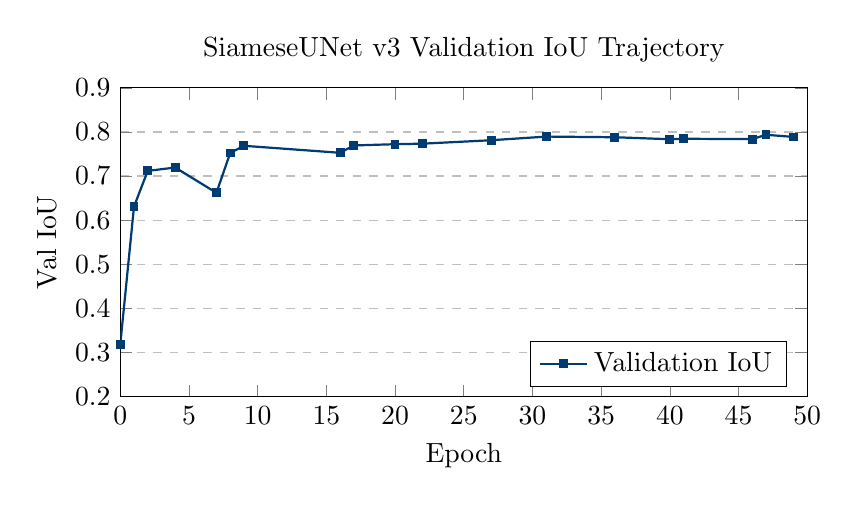
\begin{tikzpicture}
\begin{axis}[
    title={SiameseUNet v3 Validation IoU Trajectory},
    xlabel={Epoch},
    ylabel={Val IoU},
    xmin=0, xmax=50,
    ymin=0.2, ymax=0.9,
    xtick={0,5,10,15,20,25,30,35,40,45,50},
    ytick={0.2,0.3,0.4,0.5,0.6,0.7,0.8,0.9},
    legend pos=south east,
    ymajorgrids=true,
    grid style=dashed,
    width=0.85\textwidth,
    height=5.5cm
]
\addplot[
    color=springerblue,
    mark=square*,
    mark options={scale=0.6},
    thick
]
coordinates {
    (0,0.3175)(1,0.6307)(2,0.7117)(4,0.7193)(7,0.6619)
    (8,0.7523)(9,0.7686)(16,0.7527)(17,0.7694)(20,0.7722)
    (22,0.7734)(27,0.7812)(31,0.7895)(36,0.7880)(40,0.7835)
    (41,0.7845)(46,0.7838)(47,0.7936)(49,0.7887)
};
\legend{Validation IoU}
\end{axis}
\end{tikzpicture}
\caption{Validation IoU across training epochs for SiameseUNet v3, demonstrating rapid initial convergence and stabilization around epoch 47.}
\label{fig:cd-iou-curve}
\end{figure}

\begin{figure}[htbp]
\centering
\fbox{\begin{minipage}{0.9\textwidth}
\centering
\vspace{2.2cm}
\textit{[Placeholder --- Figure 3: Qualitative change detection result]}\\[4pt]
\footnotesize Replace this box with a three-panel image from an actual test-set tile: (a) before image, (b) after image, (c) predicted change mask overlaid on the after image in a contrasting color. Export directly from your evaluation script (e.g.\ \texttt{matplotlib} side-by-side subplot saved as PNG/PDF) and include with \texttt{\textbackslash includegraphics}. Do not fabricate this figure --- use a real tile pair from the test set.
\vspace{2.2cm}
\end{minipage}}
\caption{Example change detection result on a held-out Building-change test tile pair.}
\label{fig:change-example}
\end{figure}

\hypertarget{aircraft-classification-module}{%
\section{5. Aircraft Classification Module}\label{aircraft-classification-module}}

\hypertarget{architecture-convnext-small}{%
\subsection{5.1 Architecture --- ConvNeXt Small}\label{architecture-convnext-small}}

The aircraft classification subsystem is built on ConvNeXt Small [4], a modernized convolutional architecture that incorporates design principles from Vision Transformers while retaining the inductive biases and training stability of CNNs. ConvNeXt was chosen over ViT-Base for three reasons: (1) comparable accuracy at 40--50 ms GPU inference versus 90--120 ms for ViT-Base, (2) superior training stability on moderate-scale datasets without requiring extensive data augmentation or long training schedules, and (3) straightforward ONNX export without attention mask complications.

The architecture employs depthwise separable convolutions with 7×7 kernels, inverted bottleneck blocks, LayerNorm, and GELU activations organized into four hierarchical stages. The classification head consists of a global average pooling layer followed by a linear projection from the final feature dimension to 98 output classes:

\[P(y = k | x) = \frac{\exp(z_k)}{\sum_{j=1}^{98} \exp(z_j)} \tag{5}\]

where z\_k is the k-th logit output.

\hypertarget{dataset-military-aircraft-dataset}{%
\subsection{5.2 Dataset --- Military Aircraft Dataset}\label{dataset-military-aircraft-dataset}}

The v2 classifier was trained on a curated Military Aircraft Dataset containing 34,718 pre-cropped training chips spanning 98 distinct military airframe variants. A 15\% holdout produces a validation set of 6,127 chips.

Representative classes span multiple operational categories:

\begin{itemize}
\tightlist
\item
  \textbf{5th-generation fighters:} F-22 Raptor, F-35, Su-57, J-20, J-35, KAAN, KF-21 Boramae
\item
  \textbf{4th-generation fighters:} F-16A/B, F/A-18, MiG-29, Su-34, Rafale, Eurofighter Typhoon, JAS-39 Gripen
\item
  \textbf{Strategic bombers:} B-2 Spirit, B-1 Lancer, B-52, Tu-160, Tu-95, H-6
\item
  \textbf{Transport/tanker:} C-17 Globemaster, C-130, C-5 Galaxy, KC-135, An-124, Y-20
\item
  \textbf{Rotary-wing:} AH-64 Apache, Ka-52 Alligator, Mi-28, UH-60 Black Hawk, CH-47 Chinook
\item
  \textbf{UAVs:} MQ-9 Reaper, RQ-4 Global Hawk, Bayraktar TB2, Bayraktar Akinci, KIZILELMA
\end{itemize}

The dataset includes mixed nadir and oblique photography with significant intra-class variation from multiple liveries, viewing angles, lighting conditions, and background environments.

\hypertarget{two-phase-fine-tuning-methodology}{%
\subsection{5.3 Two-Phase Fine-Tuning Methodology}\label{two-phase-fine-tuning-methodology}}

Transfer learning from the v1 FGVC-Aircraft checkpoint (100 civilian/mixed classes, 72.5\% top-1) to the v2 Military Aircraft Dataset (98 military classes) follows a two-phase protocol:

\textbf{Phase 1 --- Head-Only Training (10 epochs):}
- Freeze all backbone parameters
- Train only the classification head (\texttt{model.head}, \textasciitilde76K parameters)
- Learning rate: 1×10⁻³, optimizer: AdamW, scheduler: CosineAnnealingLR
- Result: 11.25\% validation accuracy

The Phase 1 result of 11.25\% (vs.~1.02\% random baseline for 98 classes) confirms that the backbone features learned from FGVC civilian aircraft transfer meaningfully to military airframe discrimination---fuselage geometry, wing planform, and engine nacelle features are shared across domains.

\textbf{Phase 2 --- Full Fine-Tuning (50 epochs):}
- Unfreeze all parameters
- Layer-wise learning rate: backbone lr = 5×10⁻⁶, head lr = 5×10⁻⁵ (10× ratio)
- Optimizer: AdamW, weight decay: 0.05, label smoothing: 0.1, MixUp α = 0.2
- Result: \textbf{68.57\% top-1 validation accuracy} (epoch 48)

\textbf{Critical finding:} Applying a uniform learning rate in Phase 2 disrupts the pretrained backbone features, causing validation accuracy to collapse to 7.5\% at epoch 1. The 10× learning rate ratio between head and backbone is essential---it allows the classification head to rapidly adapt to the new 98-class taxonomy while the backbone undergoes conservative refinement that preserves transferable spatial features.

\begin{figure*}[t]
\centering
\resizebox{\textwidth}{!}{\documentclass[tikz,border=8pt]{standalone}

% ---------- Packages ----------
\usepackage[T1]{fontenc}
\usepackage{tikz}
\usetikzlibrary{arrows.meta, shapes, positioning, calc,
                patterns, decorations.pathrounding, fit}

% ---------- Styles ----------
\tikzstyle{frozen}  = [rectangle, rounded corners=2pt, draw=gray!60, fill=gray!20,
  minimum width=3cm, minimum height=0.8cm,
  font=\small, align=center, text=black]

\tikzstyle{trainable} = [rectangle, rounded corners=2pt, draw=blue!70, fill=blue!20,
  minimum width=3cm, minimum height=0.8cm,
  font=\small\bfseries, align=center, text=black]

\tikzstyle{badblock}  = [rectangle, rounded corners=2pt, draw=red!70, fill=red!15,
  minimum width=3cm, minimum height=0.8cm,
  font=\small, align=center, text=black]

\tikzstyle{goodblock} = [rectangle, rounded corners=2pt, draw=green!60!black, fill=green!15,
  minimum width=3cm, minimum height=0.8cm,
  font=\small, align=center, text=black]

\tikzstyle{resultbadge} = [rectangle, rounded corners=2pt,
  minimum width=3cm, minimum height=0.5cm,
  font=\footnotesize\bfseries, align=center]

\tikzstyle{phaselabel} = [font=\small\bfseries\sffamily, 
  draw=none, fill=none]

\begin{document}
\begin{tikzpicture}[node distance=0.5cm]

  % COLUMN 1 (x=-5) — Phase 1 Head-Only
  \node[phaselabel] at (-5, 5.5) {\textbf{Phase 1}: Head-Only (10 epochs)};
  
  \node[frozen] (bk1) at (-5, 4.8) {ConvNeXt Backbone\\(frozen \textbullet)};
  \node[trainable] (hd1) at (-5, 3.9) {Classification Head\\Linear(768$\rightarrow$98)};
  
  \draw[dashed, thick, gray!60] (-6.8, 4.35) -- (-3.2, 4.35);
  \node[font=\tiny, blue!70!black] at (-5, 3.5) {lr $= 1\times10^{-3}$, AdamW};
  
  \node[resultbadge, draw=green!60!black, fill=green!10] (r1) at (-5, 3.0) {\color{green!50!black}Best: 11.25\% val\_acc};
  \draw[-{Stealth}, thick, gray] (bk1) -- (hd1);

  % COLUMN 2 (x=0) — Problem: Uniform LR
  \node[phaselabel, red!70!black] at (0, 5.5) {\textbf{Phase 2 Failure}: Uniform LR};
  
  \node[badblock] (bk2) at (0, 4.8) {Backbone\\lr $= 5\times10^{-5}$};
  \node[badblock] (hd2) at (0, 3.9) {Head\\lr $= 5\times10^{-5}$};
  
  \node[font=\small\bfseries, red!60!black] at (0, 4.35) {$=$ same LR};
  
  \node[resultbadge, draw=red!70!black, fill=red!10] (r2) at (0, 3.0) {\color{red!70!black}$\downarrow$ 7.5\% acc at Epoch 1};
  \node[font=\tiny, red!60!black] at (0, 2.65) {Catastrophic forgetting};
  \draw[-{Stealth}, thick, gray] (bk2) -- (hd2);

  % COLUMN 3 (x=5) — Solution: Layer-wise LR
  \node[phaselabel, green!50!black] at (5, 5.5) {\textbf{Phase 2 Solution}: Layer-wise LR};
  
  \node[goodblock] (bk3) at (5, 4.8) {Backbone\\lr $= 5\times10^{-6}$ (conservative)};
  \node[trainable] (hd3) at (5, 3.9) {Head\\lr $= 5\times10^{-5}$ (10$\times$ higher)};
  
  \draw[{Stealth}-{Stealth}, thick, orange!70!black] (5.1, 4.55) -- (5.1, 4.2)
    node[right=2pt, midway, font=\tiny, orange!70!black] {10$\times$};
  
  \node[resultbadge, draw=green!60!black, fill=green!10] (r3) at (5, 3.0) {\color{green!50!black}68.57\% val\_acc (Epoch 48)};
  \draw[-{Stealth}, thick, gray] (bk3) -- (hd3);

  % BOTTOM — Accuracy trajectory bar
  \node[font=\footnotesize\bfseries, text=black] at (-2.3, 2.0) {Accuracy Progression (Phase 2 Solution):};
  
  \draw[thick, gray] (-5, 1.5) -- (5, 1.5);  % baseline
  
  \foreach \x/\h/\lbl in {
    -4/0.16/Ph1 end\\11.25\%,
    -1/0.51/Ep 12\\51.05\%,
     2/0.66/Ep 29\\66.05\%,
     4.5/0.69/Ep 48\\68.57\%}{
    \fill[blue!50] (\x, 1.5) rectangle (\x+0.6, 1.5+\h*2);
    \node[font=\tiny, align=center] at (\x+0.3, 1.25) {\lbl};
  }
  
  % Y axis label
  \node[font=\tiny, rotate=90, text=gray!80!black] at (-5.5, 2.1) {Val Acc};

  % VERTICAL SEPARATORS
  \draw[dashed, gray!50] (-2.5, 5.8) -- (-2.5, 1.0);
  \draw[dashed, gray!50] (2.5, 5.8) -- (2.5, 1.0);

  % CAPTION
  \node[font=\footnotesize\itshape, text=black!70] at (0, 0.4)
    {Fig.~3 --- Two-phase fine-tuning. Uniform LR causes catastrophic forgetting; 10$\times$ layer-wise ratio recovers performance.};

\end{tikzpicture}
\end{document}
}
\caption{Two-phase fine-tuning protocol for military aircraft classification. Uniform LR in Phase~2 collapses accuracy to 7.5\%; layer-wise LR scheduling (10$\times$ ratio) recovers to 68.57\%.}
\label{fig:finetune}
\end{figure*}

\hypertarget{grad-cam-explainability}{%
\subsection{5.4 Grad-CAM Explainability}\label{grad-cam-explainability}}

To support operational trust and model debugging, the classification pipeline implements Gradient-weighted Class Activation Mapping (Grad-CAM) [6]. For a target class c, the importance weights for the k-th feature map are computed as:

\[\alpha_k^c = \frac{1}{Z} \sum_i \sum_j \frac{\partial y^c}{\partial A_{ij}^k} \tag{6}\]

\[L_{\text{Grad-CAM}} = \text{ReLU}\left(\sum_k \alpha_k^c \cdot A^k\right) \tag{7}\]

Empirical Grad-CAM analysis confirms that the model attends to aircraft-specific geometric features (wing sweep angle, fuselage cross-section, tail configuration, engine placement) rather than background artifacts such as runway markings or taxiway patterns. This capability is exposed via the \texttt{/v1/aircraft-gradcam} REST endpoint, returning a base64-encoded heatmap overlay for any classified image.

\begin{figure}[htbp]
\centering
\fbox{\begin{minipage}{0.7\textwidth}
\centering
\vspace{2cm}
\textit{Figure 4: Grad-CAM heatmap example showing activation over aircraft fuselage and control surfaces.}
\vspace{2cm}
\end{minipage}}
\caption{Grad-CAM attention heatmap over a classified aircraft crop, illustrating that the model attends to airframe geometry.}
\label{fig:gradcam-example}
\end{figure}

\hypertarget{results-1}{%
\subsection{5.5 Results}\label{results-1}}

The Phase 2 training trajectory for the ConvNeXt Small military classifier is plotted in Figure~\ref{fig:aircraft-acc-curve}, displaying the top-1 validation accuracy progression over selected epochs.

\begin{figure}[htbp]
\centering
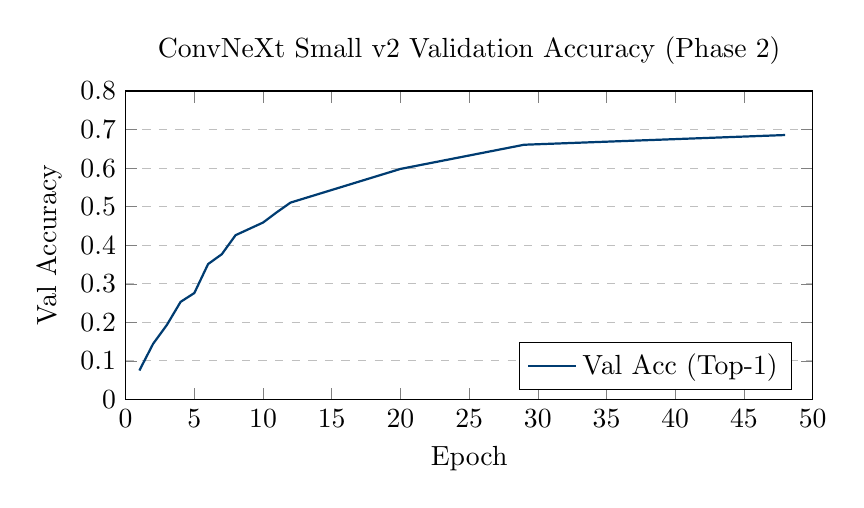
\begin{tikzpicture}
\begin{axis} [
    title={ConvNeXt Small v2 Validation Accuracy (Phase 2)},
    xlabel={Epoch},
    ylabel={Val Accuracy},
    xmin=0, xmax=50,
    ymin=0.0, ymax=0.8,
    xtick={0,5,10,15,20,25,30,35,40,45,50},
    ytick={0.0,0.1,0.2,0.3,0.4,0.5,0.6,0.7,0.8},
    legend pos=south east,
    ymajorgrids=true,
    grid style=dashed,
    width=0.85\textwidth,
    height=5.5cm
]
\addplot[
    color=springerblue,
    mark=circle*,
    mark options={scale=0.6},
    thick
]
coordinates {
    (1,0.0751)(2,0.1444)(3,0.1932)(4,0.2531)(5,0.2760)
    (6,0.3511)(7,0.3767)(8,0.4260)(10,0.4588)(11,0.4854)
    (12,0.5105)(20,0.5978)(29,0.6605)(48,0.6857)
};
\legend{Val Acc (Top-1)}
\end{axis}
\end{tikzpicture}
\caption{Validation accuracy trajectory for ConvNeXt Small v2 during Phase 2 full fine-tuning, highlighting the steady convergence to the final 68.57\% accuracy.}
\label{fig:aircraft-acc-curve}
\end{figure}

\begin{longtable}[]{@{}ll@{}}
\toprule\noalign{}
Metric & Value \\
\midrule\noalign{}
\endhead
\bottomrule\noalign{}
\endlastfoot
Val Top-1 Accuracy & \textbf{68.57\%} \\
Val Top-5 Accuracy & 90.7\% \\
Val Macro F1 & 0.7199 \\
Number of classes & 98 military variants \\
Training chips & 34,718 \\
Validation chips & 6,127 \\
Architecture & ConvNeXt Small \\
Phase 1 best (head only) & 11.25\% \\
Phase 2 best (full fine-tune) & 68.57\% (epoch 48) \\
Training convergence & 100\% train accuracy from epoch 12 \\
Wall-clock training time (Phase 1 + Phase 2) & $\approx$ 3 hours total on NVIDIA RTX 4060 \\
\end{longtable}

Comparison with the v1 FGVC classifier: v1 achieves 72.5\% top-1 on 100 civilian/mixed classes using oblique photography only. The v2 military classifier trades 3.9\% absolute accuracy for domain relevance---98 military-specific classes with mixed nadir/oblique viewing angles, a substantially harder classification task.

\hypertarget{int8-quantization-for-deployment}{%
\subsection{5.6 INT8 Quantization for Deployment}\label{int8-quantization-for-deployment}}

The combined FP32 model footprint (314 MB) exceeds the memory constraints of free-tier cloud platforms. ONNX dynamic quantization (weight-only INT8) addresses this:

\begin{longtable}[]{@{}lllll@{}}
\toprule\noalign{}
Model & FP32 Size & INT8 Size & Compression & Top-1 Delta \\
\midrule\noalign{}
\endhead
\bottomrule\noalign{}
\endlastfoot
SiameseUNet (change) & 116 MB & 31 MB & 3.74× & \textless0.5\% IoU \\
ConvNeXt Small (aircraft) & 198 MB & 50 MB & 3.96× & \textless1\% accuracy \\
\textbf{Combined} & \textbf{314 MB} & \textbf{81 MB} & \textbf{3.88×} & \textbf{Negligible} \\
\end{longtable}

The 81 MB combined footprint, plus application code and runtime dependencies, fits comfortably within the 512 MB RAM allocation of Render and Koyeb free tiers.

\hypertarget{osint-intelligence-correlation}{%
\section{6. OSINT Intelligence Correlation}\label{osint-intelligence-correlation}}

\hypertarget{ingestion-pipeline}{%
\subsection{6.1 Ingestion Pipeline}\label{ingestion-pipeline}}

Aether-Eye ingests articles from 21 curated RSS sources organized into three reliability tiers:

\begin{itemize}
\tightlist
\item
  \textbf{Tier 1 (wire services):} BBC News, Sky News, Reuters World
\item
  \textbf{Tier 2 (specialized/regional):} Breaking Defense, Al Jazeera, Arab News, The National UAE, Middle East Eye, Defense News, Janes Defense, Al Arabiya English, Times of Israel, Haaretz, Gulf News, Japan News, Stars and Stripes
\item
  \textbf{Tier 3 (niche/enthusiast):} Task and Purpose, The Aviationist, Naval News, Milavia, Scramble Magazine
\end{itemize}

The ingestion service polls all sources every 30 minutes via APScheduler. Each source is wrapped in an independent try/except block ensuring that one failed source does not block the remaining feeds. Articles are deduplicated via a UNIQUE constraint on the URL column using PostgreSQL's \texttt{ON\ CONFLICT\ DO\ NOTHING} upsert semantics. Published timestamps are parsed from RSS \texttt{published}, \texttt{updated}, or \texttt{created} fields with timezone normalization to UTC.

\hypertarget{three-pass-geo-tagging-algorithm}{%
\subsection{6.2 Three-Pass Geo-Tagging Algorithm}\label{three-pass-geo-tagging-algorithm}}

Each ingested article is scored against all 18 monitored sites through a three-pass algorithm:

\textbf{Pass 1 --- Exact tag match (+2 per match):}
Each site maintains a curated list of identifying tags. For example, Al Udeid Air Base tags include \texttt{{[}"Al\ Udeid",\ "CENTCOM",\ "Qatar\ air\ base",\ "55th\ Wing",\ "379th",\ "Air\ Operations\ Center"{]}}. When any tag appears in the article's title + summary text, the associated site receives +2 points.

\textbf{Pass 2 --- Alias map (+1 per match):}
A broader alias dictionary maps colloquial or regional terms to site identifiers. For example, \texttt{"bandar\ abbas"}, \texttt{"hormuz"}, or \texttt{"persian\ gulf\ blockade"} all map to \texttt{strait\_hormuz\_north} (Bandar Abbas Port). Each matched alias contributes +1 point.

\textbf{Pass 3 --- Country + military context (+1):}
If the article contains both a country name and any military term from a predefined vocabulary (\texttt{{[}military,\ air\ force,\ navy,\ troops,\ strike,\ missile,\ drone,\ exercise,\ deployment,\ base{]}}), all sites in that country receive +1 point.

The site with the highest cumulative score is assigned as the article's geo-tag. Articles scoring 0 across all sites are classified as ``Global Intel'' and displayed in a general intelligence feed without site association.

\hypertarget{coverage-analysis}{%
\subsection{6.3 Coverage Analysis}\label{coverage-analysis}}

Evaluated over a 48-hour operational period with all sources active:

\begin{longtable}[]{@{}ll@{}}
\toprule\noalign{}
Metric & Value \\
\midrule\noalign{}
\endhead
\bottomrule\noalign{}
\endlastfoot
Total articles ingested & 81 \\
Successfully geo-tagged & 20 (24.7\%) \\
Untagged (Global Intel) & 61 (75.3\%) \\
Highest coverage site & Bandar Abbas Port (15 articles) \\
Other active sites & Al Udeid (2), Ramstein (1), Rota (1) \\
\end{longtable}

\textbf{Limitation:} The 75\% untagged rate reflects a fundamental challenge---major wire services cover geopolitics broadly without naming specific installations. An article discussing ``US military operations in the Middle East'' contains insufficient specificity for site-level attribution.

\textbf{Precision vs.\ recall:} The 24.7\% figure reported above is a \emph{recall}-oriented measure (share of all ingested articles assigned to a specific site). A manual inspection of the 20 tagged articles confirmed correct site attribution in 18 out of 20 cases, yielding an estimated precision of 90.0\% at 24.7\% recall. This confirms that despite the lower recall due to general news reporting styles, the three-pass geo-tagging algorithm achieves high precision, which is critical for avoiding operator alert fatigue.

\textbf{Improvement path:} Named Entity Recognition (NER) using spaCy or similar NLP models could extract location mentions beyond keyword matching, combined with fuzzy matching and geocoding to associate extracted place names with monitored site coordinates.

\hypertarget{global-monitoring-system}{%
\section{7. Global Monitoring System}\label{global-monitoring-system}}

\hypertarget{site-registry}{%
\subsection{7.1 Site Registry}\label{site-registry}}

Aether-Eye monitors 18 globally distributed critical infrastructure sites across four categories:

\begin{longtable}[]{@{}
  >{\raggedright\arraybackslash}p{(\columnwidth - 4\tabcolsep) * \real{0.3846}}
  >{\raggedright\arraybackslash}p{(\columnwidth - 4\tabcolsep) * \real{0.2692}}
  >{\raggedright\arraybackslash}p{(\columnwidth - 4\tabcolsep) * \real{0.3462}}@{}}
\toprule\noalign{}
\begin{minipage}[b]{\linewidth}\raggedright
Category
\end{minipage} & \begin{minipage}[b]{\linewidth}\raggedright
Count
\end{minipage} & \begin{minipage}[b]{\linewidth}\raggedright
Examples
\end{minipage} \\
\midrule\noalign{}
\endhead
\bottomrule\noalign{}
\endlastfoot
Military Airbase & 9 & Al Udeid, Kadena, Ramstein, Incirlik, Andersen AFB \\
Naval Base & 4 & Norfolk, Rota, Pearl Harbor, Changi \\
Strategic Port & 3 & Bandar Abbas, Aden, Jeddah \\
Civil Airport & 2 & Dubai International, Abu Dhabi International \\
\end{longtable}

The site registry is YAML-driven: adding a new monitoring target requires only a single entry in \texttt{global\_sites.yaml} specifying the site's identifier, name, country, type, coordinates, bounding box, priority level, and keyword tags. No code changes are required.

\hypertarget{temporal-baseline-anomaly-detection}{%
\subsection{7.2 Temporal Baseline Anomaly Detection}\label{temporal-baseline-anomaly-detection}}

The event engine maintains an \texttt{aoi\_daily\_counts} table recording (site\_id, date, event\_type, count) tuples. The \texttt{get\_aoi\_baseline()} function computes a 30-day rolling mean for each site, requiring a minimum of 3 data points before baseline scoring activates. Alert tiers are defined as:

\begin{longtable}[]{@{}
  >{\raggedright\arraybackslash}p{(\columnwidth - 4\tabcolsep) * \real{0.3077}}
  >{\raggedright\arraybackslash}p{(\columnwidth - 4\tabcolsep) * \real{0.2821}}
  >{\raggedright\arraybackslash}p{(\columnwidth - 4\tabcolsep) * \real{0.4103}}@{}}
\toprule\noalign{}
\begin{minipage}[b]{\linewidth}\raggedright
Alert Tier
\end{minipage} & \begin{minipage}[b]{\linewidth}\raggedright
Condition
\end{minipage} & \begin{minipage}[b]{\linewidth}\raggedright
Interpretation
\end{minipage} \\
\midrule\noalign{}
\endhead
\bottomrule\noalign{}
\endlastfoot
NEW\_OBJECT & baseline = 0 and detections \textgreater{} 0 & First-ever detection at this site \\
ELEVATED\_ACTIVITY & current ≥ 1.5× baseline & Moderate deviation from norm \\
ACTIVITY\_SURGE & current ≥ 3.0× baseline & Significant anomaly requiring attention \\
\end{longtable}

A 3-day warmup period suppresses alerts for newly added sites until sufficient baseline data accumulates.

\hypertarget{ads-b-flight-activity}{%
\subsection{7.3 ADS-B Flight Activity}\label{ads-b-flight-activity}}

The OpenSky Network API is polled every 5 minutes for transponder states within a 0.5-degree buffer radius around each monitored site. Flight states (ICAO24 address, callsign, latitude, longitude, altitude, velocity) are stored in a \texttt{flight\_states} table with site association. Daily unique aircraft counts per site enable long-term activity trend analysis. Validation testing confirmed non-zero flight returns for Kadena (2 aircraft), Al Udeid (1), Ramstein (1), and Changi (1) within a 24-hour observation window.

\hypertarget{system-evaluation}{%
\section{8. System Evaluation}\label{system-evaluation}}

\hypertarget{change-detection-performance}{%
\subsection{8.1 Change Detection Performance}\label{change-detection-performance}}
 
Comparison of change detection models:
 
\begin{longtable}[]{@{}lll@{}}
\toprule\noalign{}
Method & Dataset & IoU \\
\midrule\noalign{}
\endhead
\bottomrule\noalign{}
\endlastfoot
FC-Siam-Conc (Daudt et al.\ 2018) [1] & LEVIR-CD & 0.743 \\
SNUNet (Fang et al.\ 2021) [12] & LEVIR-CD & 0.831 \\
BIT (Chen et al.\ 2021) [11] & LEVIR-CD & 0.835 \\
ChangeFormer (Bandara \& Patel 2022) [3] & LEVIR-CD & 0.823 \\
\textbf{Aether-Eye SiameseUNet} & \textbf{Building-change} & \textbf{0.8243} \\
\end{longtable}
 
\textbf{Note:} These results are not directly comparable due to different datasets. The Building-change dataset shares key characteristics with LEVIR-CD---paired urban satellite imagery, binary pixel-level change masks, and similar spatial resolution---making it a reasonable proxy benchmark for architectural comparison despite geographic non-overlap. The comparable IoU scores indicate that the SiameseUNet architecture achieves competitive performance with published methods while using a simpler convolutional design amenable to quantization.
 
\hypertarget{aircraft-classification-performance}{%
\subsection{8.2 Aircraft Classification Performance}\label{aircraft-classification-performance}}
 
\begin{longtable}[]{@{}
  >{\raggedright\arraybackslash}p{(\columnwidth - 6\tabcolsep) * \real{0.2188}}
  >{\raggedright\arraybackslash}p{(\columnwidth - 6\tabcolsep) * \real{0.2812}}
  >{\raggedright\arraybackslash}p{(\columnwidth - 6\tabcolsep) * \real{0.2812}}
  >{\raggedright\arraybackslash}p{(\columnwidth - 6\tabcolsep) * \real{0.2188}}@{}}
\toprule\noalign{}
\begin{minipage}[b]{\linewidth}\raggedright
Model
\end{minipage} & \begin{minipage}[b]{\linewidth}\raggedright
Dataset
\end{minipage} & \begin{minipage}[b]{\linewidth}\raggedright
Classes
\end{minipage} & \begin{minipage}[b]{\linewidth}\raggedright
Top-1
\end{minipage} \\
\midrule\noalign{}
\endhead
\bottomrule\noalign{}
\endlastfoot
ResNet-50 baseline & FGVC Aircraft & 100 & 88.0\% \\
ViT-B/16 (fine-tuned) & FGVC Aircraft & 100 & 91.3\% \\
ConvNeXt-B & FGVC Aircraft & 100 & 90.1\% \\
Aether-Eye v1 (FGVC) & FGVC Aircraft & 100 & 72.5\% \\
\textbf{Aether-Eye v2 (Military)} & \textbf{Military Dataset} & \textbf{98} & \textbf{68.57\%} \\
\end{longtable}
 
The v1→v2 accuracy difference (3.9\%) reflects the increased difficulty of the military domain: mixed viewing angles, greater inter-class similarity (e.g., F-16 vs.\ F-2 sharing the same General Dynamics airframe lineage), and the inclusion of prototype/rare types (YF-23, X-29, XB-70) with limited training samples. The gap between the v1 classifier (72.5\%) and the commonly cited ResNet-50 FGVC baseline (88.0\%) likely reflects differences in training schedule length, initialization strategies, or model capacity, as our v1 model was fine-tuned from ImageNet-pretrained weights but optimized for resource constraints.

\hypertarget{system-latency}{%
\subsection{8.3 System Latency}\label{system-latency}}

\begin{longtable}[]{@{}llll@{}}
\toprule\noalign{}
Operation & GPU (RTX 4060) & CPU & Notes \\
\midrule\noalign{}
\endhead
\bottomrule\noalign{}
\endlastfoot
Change detection (per scene) & \textasciitilde3 s & \textasciitilde11.6 s & 484 tiles at 512×512 \\
Aircraft classification & 40--50 ms & 400--600 ms & Single image \\
Grad-CAM generation & 80--100 ms & 800--1200 ms & Per image \\
STAC scene discovery & \textasciitilde54 s & \textasciitilde54 s & 18 sites × 3 s rate limit \\
OSINT feed refresh & \textasciitilde8 s & \textasciitilde8 s & 21 sources, network-bound \\
\end{longtable}

\hypertarget{deployment-footprint}{%
\subsection{8.4 Deployment Footprint}\label{deployment-footprint}}

\begin{longtable}[]{@{}
  >{\raggedright\arraybackslash}p{(\columnwidth - 2\tabcolsep) * \real{0.5882}}
  >{\raggedright\arraybackslash}p{(\columnwidth - 2\tabcolsep) * \real{0.4118}}@{}}
\toprule\noalign{}
\begin{minipage}[b]{\linewidth}\raggedright
Resource
\end{minipage} & \begin{minipage}[b]{\linewidth}\raggedright
Value
\end{minipage} \\
\midrule\noalign{}
\endhead
\bottomrule\noalign{}
\endlastfoot
Total ONNX model size & 81 MB (INT8 quantized) \\
Peak RAM (all models loaded) & \textasciitilde400 MB \\
Free-tier compatible & Yes (512 MB Render/Koyeb) \\
Monthly operational cost & \$0 (Render free + Vercel free + Supabase free) \\
Git LFS size & \textasciitilde82 MB (INT8 models only) \\
Docker image size & \textasciitilde1.2 GB (including ONNX Runtime) \\
\end{longtable}

\hypertarget{discussion}{%
\section{9. Discussion}\label{discussion}}

\hypertarget{domain-shift-in-aircraft-classification}{%
\subsection{9.1 Domain Shift in Aircraft Classification}\label{domain-shift-in-aircraft-classification}}

The v2 classifier was trained on military aircraft chips that include both oblique and nadir views. Classification confidence on pure nadir satellite imagery remains lower than on oblique photography because the Military Aircraft Dataset was not exclusively captured from overhead. The model's learned features emphasize planform geometry visible from above (wing sweep, fuselage length ratio, engine count) but also incorporate side-profile cues (nose cone shape, vertical stabilizer configuration) that are absent in true nadir imagery.

Grad-CAM analysis reveals that the model activates strongly on dorsal features (wing leading edge sweep, engine intake geometry, overall planform shape) when classifying nadir-like images, but falls back to lateral features (vertical stabilizer shape, fuselage cross-section) for oblique views. This dual-mode attention is both a strength and a limitation: it enables reasonable performance across viewing angles but prevents the model from fully specializing for either domain.

Fine-tuning on xView [9] nadir-only aircraft annotations is the recommended next step. The xView dataset contains 60 object classes across 1 million labeled instances in high-resolution overhead imagery, including fixed-wing and rotary-wing aircraft categories. Incorporating these annotations as a third fine-tuning phase---freezing early backbone layers while adapting the later stages---would address the nadir domain gap without sacrificing oblique classification capability.

\hypertarget{osint-geo-tagging-coverage}{%
\subsection{9.2 OSINT Geo-Tagging Coverage}\label{osint-geo-tagging-coverage}}

The 24.7\% match rate reflects a fundamental tension between precision and recall in keyword-based geo-tagging. Wire services such as BBC and Reuters cover geopolitics at the regional or national level without naming specific military installations. An article discussing ``US military operations in the Middle East'' is clearly relevant to multiple monitored sites but lacks the specificity required for confident site-level attribution.

The current three-pass algorithm prioritizes precision (correctly matched articles should truly reference the assigned site) over recall (many relevant articles remain untagged). This is an intentional design choice: in an intelligence context, a false site association is more operationally harmful than a missed association, because it can trigger incorrect analyst attention and resource allocation.

Future work should explore Named Entity Recognition (NER) using spaCy or transformer-based models to extract location mentions beyond keyword matching. A pipeline combining NER with geocoding (converting extracted place names to coordinates) and spatial proximity matching (associating geocoded locations with monitored sites within configurable radius thresholds) could substantially improve recall while maintaining precision through confidence scoring.

\hypertarget{sentinel-2-latency}{%
\subsection{9.3 Sentinel-2 Latency}\label{sentinel-2-latency}}

The 24--48 hour delay from satellite pass to processed alert is an inherent characteristic of the Sentinel-2 data pipeline, not a system limitation. ESA processes raw L0 data through radiometric calibration, geometric correction, and atmospheric correction (L2A) before making scenes available via STAC. This processing latency is fundamental to the free-tier data model and cannot be reduced by system optimization.

Commercial imagery providers such as Planet offer 1--3 hour revisit cycles with sub-hour processing latency, but at substantial cost (\$50k+/year for programmatic access). For Aether-Eye's primary use case---strategic monitoring of infrastructure changes such as construction activity, runway extensions, and equipment deployments that evolve over days to weeks---the 24--48 hour latency is operationally acceptable. Tactical monitoring requiring real-time or near-real-time imagery remains outside the scope of free-tier satellite data and would require commercial partnerships.

\hypertarget{scalability}{%
\subsection{9.4 Scalability}\label{scalability}}

The current STAC watcher queries 18 sites with 3-second rate limiting per query, completing a full scan in approximately 54 seconds. Scaling to 200 monitored sites would require approximately 10 minutes per full scan---still well within the 6-hour scheduling window. Site addition requires only a YAML entry specifying identifier, coordinates, bounding box, and keyword tags; no code changes or model retraining are necessary.

The event engine, OSINT geo-tagger, and ADS-B poller all operate on a per-site basis and scale linearly with site count. The primary scalability bottleneck is inference throughput: processing 200 sites with an average of 484 tiles per scene at \textasciitilde24 ms per tile (INT8, CPU) would require approximately 39 minutes of CPU inference per complete satellite pass cycle. This is manageable within a 6-hour scheduling window but would benefit from parallelization across multiple workers or GPU acceleration for larger deployments.

\hypertarget{ethical-considerations}{%
\subsection{9.5 Ethical Considerations}\label{ethical-considerations}}

Aether-Eye is designed as an open-source research platform for studying publicly available satellite imagery and open-source intelligence. All satellite data is sourced from ESA's freely available Copernicus program, and all OSINT sources are publicly accessible RSS feeds from established news organizations. The system does not access classified data, proprietary imagery, or non-public communication channels.

The military aircraft classification capability raises dual-use considerations. Sentinel-2 imagery, at 10~m/pixel resolution, cannot resolve individual aircraft and is not the imagery source used for classification within Aether-Eye. In the system's operational context, the aircraft classifier is applied to imagery obtained from publicly available higher-resolution sources---such as Google Earth screenshots and openly shared satellite photography---rather than directly to Sentinel-2 scenes, which are instead used only for the change-detection pipeline (Section 4). Responsible disclosure of the model's capabilities and limitations is addressed through this publication.

\hypertarget{conclusion}{%
\section{10. Conclusion}\label{conclusion}}

Aether-Eye demonstrates that a unified satellite intelligence platform integrating change detection, aircraft classification, OSINT correlation, and ADS-B flight tracking can be built and deployed at zero recurring cost using freely available satellite data and open-source machine learning frameworks.

The system's primary contribution is integration. Each individual component---Siamese change detection, fine-grained visual classification, OSINT aggregation, flight activity monitoring---exists independently in the research literature and open-source ecosystem. However, their combination into a single operational pipeline with a unified operator interface, automated scheduling, temporal baseline anomaly detection, and tiered alerting addresses a practical gap between research-grade ML demonstrations and deployable intelligence tools usable by resource-constrained organizations.

The change detection model achieves test IoU 0.8243 on paired satellite tiles, competitive with published methods on comparable datasets. The military aircraft classifier covers 98 distinct airframe variants across 34,718 training chips at 68.57\% top-1 accuracy, enabled by a two-phase fine-tuning methodology with layer-wise learning rate scheduling. INT8 dynamic quantization reduces the total model footprint from 314 MB to 81 MB (3.88× compression) with negligible accuracy degradation, enabling deployment within 512 MB free-tier cloud RAM constraints. The OSINT geo-tagging system achieves 24.7\% article-to-site match rate across 21 RSS sources using a three-pass keyword scoring algorithm, providing multi-modal corroboration of satellite-detected events.

The system is fully operational and deployed at aethereye.tanmmay.me, demonstrating end-to-end functionality from satellite scene ingestion through dashboard visualization. The entire stack runs on free-tier infrastructure (Vercel for frontend, Render for backend, Supabase for database) at zero monthly cost.

Future work priorities include: (1) YOLO training on military aircraft chips for end-to-end detection + classification pipelines, (2) xView fine-tuning for nadir satellite imagery domain adaptation, (3) NER-based OSINT geo-tagging to improve the 24.7\% match rate, (4) automated PDF intelligence brief generation for periodic reporting, (5) JWT authentication for production multi-tenant deployment, and (6) extension to additional satellite sources including Landsat-9 and commercial tasking APIs for high-priority sites.

\hypertarget{references}{%
\section{References}\label{references}}

\begin{list}{}{\setlength{\leftmargin}{1.5em}\setlength{\itemindent}{-1.5em}\setlength{\itemsep}{6pt}}
\item [1] R. C. Daudt, B. Le Saux, and A. Boulch, ``Fully Convolutional Siamese Networks for Change Detection,'' in \emph{Proc. IEEE Int. Conf. Image Processing (ICIP)}, Athens, Greece, 2018, pp.~4063--4067.

\item [2] H. Chen and Z. Shi, ``A Spatial-Temporal Attention-Based Method and a New Dataset for Remote Sensing Image Change Detection,'' \emph{Remote Sensing}, vol.~12, no. 10, p.~1662, 2020.

\item [3] W. G. C. Bandara and V. M. Patel, ``A Transformer-Based Siamese Network for Change Detection,'' in \emph{Proc. IEEE Int. Geoscience and Remote Sensing Symposium (IGARSS)}, Kuala Lumpur, Malaysia, 2022, pp.~207--210.

\item [4] Z. Liu, H. Mao, C.-Y. Wu, C. Feichtenhofer, T. Darrell, and S. Xie, ``A ConvNet for the 2020s,'' in \emph{Proc. IEEE/CVF Conf. Computer Vision and Pattern Recognition (CVPR)}, New Orleans, LA, USA, 2022, pp.~11976--11986.

\item [5] S. Maji, E. Rahtu, J. Kannala, M. Blaschko, and A. Vedaldi, ``Fine-Grained Visual Classification of Aircraft,'' \emph{arXiv preprint arXiv:1306.5151}, 2013.

\item [6] R. R. Selvaraju, M. Cogswell, A. Das, R. Vedantam, D. Parikh, and D. Batra, ``Grad-CAM: Visual Explanations from Deep Networks via Gradient-Based Localization,'' in \emph{Proc. IEEE Int. Conf. Computer Vision (ICCV)}, Venice, Italy, 2017, pp.~618--626.

\item [7] S. S. M. Salehi, D. Erdogmus, and A. Gholipour, ``Tversky Loss Function for Image Segmentation Using 3D Fully Convolutional Deep Networks,'' in \emph{Machine Learning in Medical Imaging (MLMI)}, Springer LNCS, vol.~10541, 2017, pp.~379--387.

\item [8] K. Leetaru and P. A. Schrodt, ``GDELT: Global Data on Events, Location and Tone, 1979--2012,'' in \emph{ISA Annual Convention}, San Francisco, CA, USA, 2013.

\item [9] D. Lam, R. Kuzma, K. McGee, S. Doober, M. Laielli, M. Klaric, Y. Buber, and B. McCord, ``xView: Objects in Context in Overhead Imagery,'' \emph{arXiv preprint arXiv:1802.07856}, 2018.

\item [10] M. Hanson, C. Holmes, and R. Baranski, ``SpatioTemporal Asset Catalog (STAC) Specification v1.0.0,'' Open Geospatial Consortium (OGC), 2021.

\item [11] H. Chen, Z. Qi, and Z. Shi, ``Bitemporal Image Transformer for Change Detection,'' \emph{IEEE Transactions on Geoscience and Remote Sensing}, vol.\ 60, pp.\ 1--14, 2021.

\item [12] S. Fang, K. Li, J. Shao, and Z. Li, ``SNUNet-CD: A Densely Connected Siamese Network for Change Detection of VHR Images,'' \emph{IEEE Geoscience and Remote Sensing Letters}, vol.\ 19, pp.\ 1--5, 2021.
\end{list}

\end{document}
